\documentclass{article}
\usepackage{xeCJK}
\usepackage{amsmath}
\usepackage{geometry}
\usepackage{graphicx}

\setCJKmainfont{Microsoft YaHei}
\linespread{1.5}
\setlength{\parindent}{0pt}

\begin{document}
1.\\
(1) 该正则语言的正则表达式为
\[
(a + b + \varepsilon) b a (a + b) ^ * b b (a + b + \varepsilon) + b b a    
\]
得到的 $\varepsilon - NFA$ 如下图所示
\begin{figure}[htbp]
	\centering
    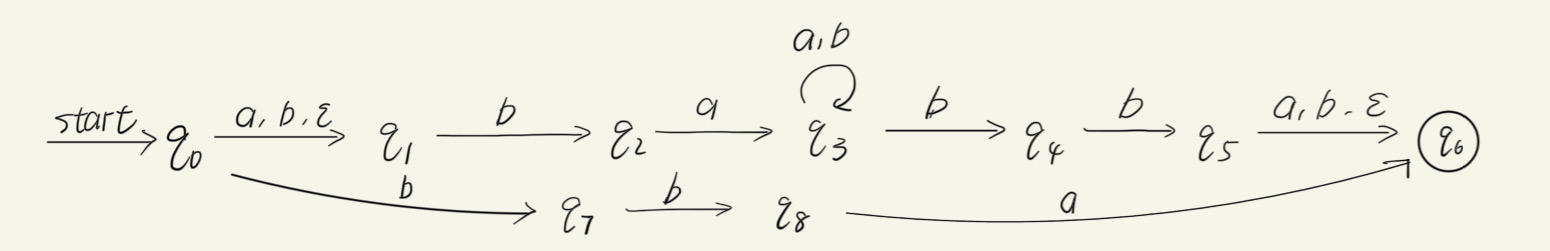
\includegraphics[width=43em,height=!]{NFA1.jpg}
	\caption{$\varepsilon - NFA$}
\end{figure}

(2) 每个状态的 $\varepsilon - \mbox{闭包}$ 如下:\\
\[
\begin{aligned}
& E\_CLOSE(q_0) = {q_0, q_1}; \\
& E\_CLOSE(q_1) = {q_1}; \\
& E\_CLOSE(q_2) = {q_2}; \\
& E\_CLOSE(q_3) = {q_3}; \\
& E\_CLOSE(q_4) = {q_4}; \\
& E\_CLSOE(q_5) = {q_5, q_6}; \\
& E\_CLOSE(q_6) = {q_6}; \\ 
& E\_CLOSE(q_7) = {q_7}; \\
& E\_CLOSE(q_8) = {q_8}; \\
\end{aligned}
\]
从而通过子集构造有:
\begin{table}[h!]
    \begin{center}
      \caption{子集构造}
      \setlength{\tabcolsep}{8mm} {
      \begin{tabular}{|l|l|l|} 
        \textbf{$subset$} & \textbf{$a$} & \textbf{$b$} \\
        \hline
        $-> A: q_0, q_1$ & $q_1$ & $q_1, q_2, q_7$ \\ 
        $B: q_1$ & $\emptyset$ & $q_2$ \\
        $C :q_1, q_2, q_7$ & $q_3$ & $q_2, q_8$ \\
        $D: q_2$ & $q_3$ & $\emptyset$ \\
        $E: q_3$ & $q_3$ & $q_3, q_4$ \\
        $F: q_2, q_8$ & $q_3, q_6$ & $\emptyset$ \\
        $G: q_3, q_4$ & $q_3$ & $q_3, q_4, q_5, q_6$ \\
        $* H: q_3, q_6$ & $q_3$ & $q_3, q_4$ \\
        $* I: q_3, q_4, q_5, q_6$ & $q_3, q_6$ & $q_3, q_4, q_5, q_6$ \\
      \end{tabular} 
      }
    \end{center}
\end{table}
\newpage
得到的 $DFA$ 如下图所示
\begin{figure}[htbp]
	\centering
    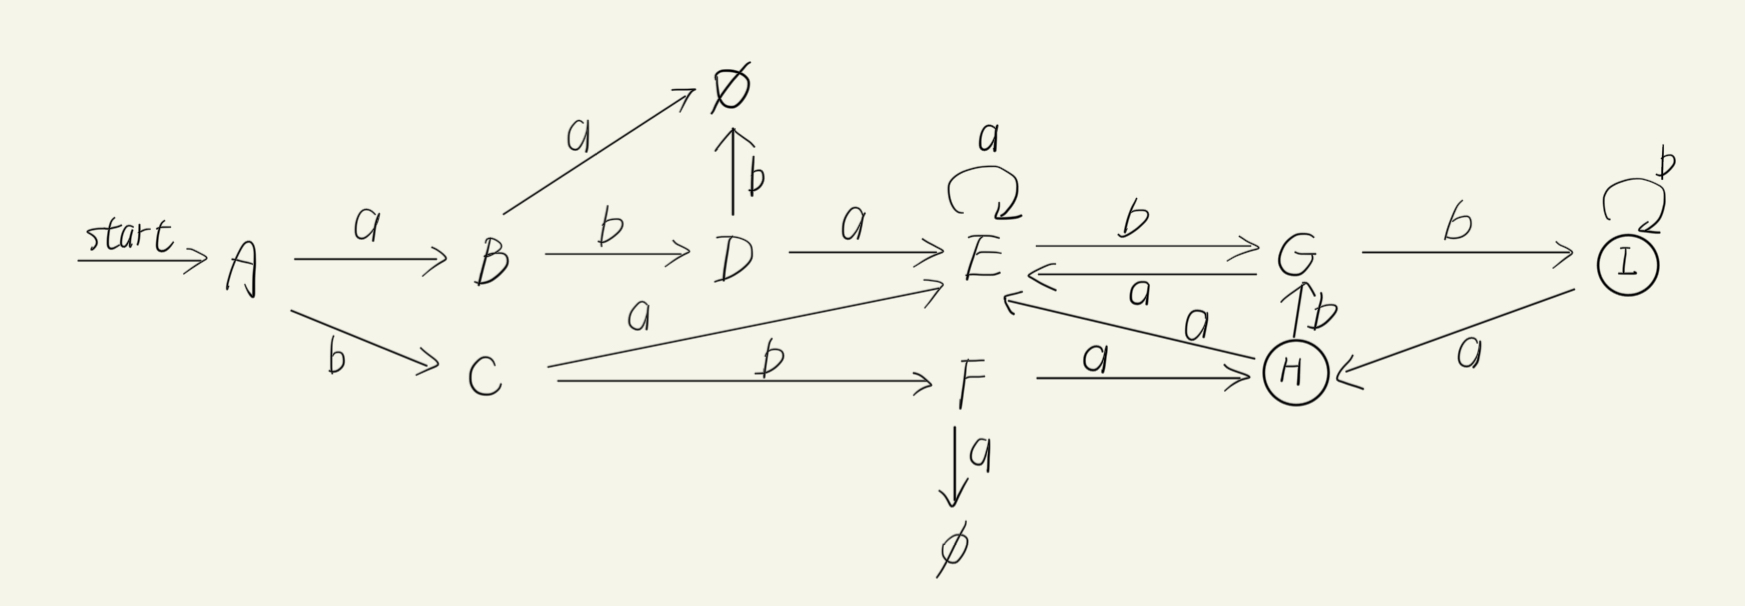
\includegraphics[width=43em,height=!]{NFA2.jpg}
	\caption{$DFA$}
\end{figure}
\\
2.$L$ 不是正则语言。\\
证明:假设 $L$ 是正则语言,取 $\omega = a^{2k - 1}b^{2k}$,其中 $k \geq 2, k \in R^{+}$,\\
$2k - 1$ 和 $2k$ 的最大公约数为 $1$,故 $\omega \in L$. \\
取 
\[
    x = a^{2k - 1 - n},\; y = a^{n} b^{n + 1},\; z = b^{2k - 1 - n},\; N = 4k - 3,
\]
则 $|\omega| = 4k - 1 \geq N,\; |xy| = 2k - 1 \leq N $, \\
取 $m = 0$,则 $xy^{m}z = xy^{0}z = a^{2k - 1 - n}b^{2k - 1 - n}$,\\
而 $|xy| = 2k + n \leq N = 4k - 3$,故有 $n \leq 2k - 3$,从而 $2k - 1 - n \geq 2$,
即 $2k - 1 - n$ 和 $2k - 1 -n$ 有大于 $1$ 的公约数,故 $xy^{0}z \notin L$,由泵引理 $xy^{0}z \in L$,矛盾,故 $L$ 不是正则语言。\\
\end{document}3